\documentclass{book}
\usepackage[spanish]{babel}
\usepackage[utf8]{inputenc} 
\usepackage[T1]{fontenc}
\usepackage{lmodern}
\usepackage{graphicx}
\usepackage{amsmath}
\usepackage{xcolor}
\usepackage{verbatim} 
\usepackage{enumerate} % enumerados

%\usepackage[natbibapa]{apacite}
%\usepackage[hyperpageref]{backref}
%\usepackage[alf]{abntex2cite}

\begin{document}
%\chapter{Introdución}
%	\section{Motivación}
%	\section{Planteamiento del problema}
%	\section{Hipótesis}
%	\section{Objetivos}
%	\section{Descripción del documento}
\chapter{Antecedentes}
	\section{Robots bípedos}
		\subsection{Sistema con extremidades}
Citando a \cite{siciliano2016springer}	\textit{Limbed system} es un robot móvil que debe tener un cuerpo y al menos una pierna (extremidad inferior) para apoyarse e impulsarse.

	Una de sus piernas interactúa con el medio con su actuador final (pie) y 			puede tener un arbitrario número de brazos (extremidades superiores) para 					manipular objetos con sus actuadores finales (manos). \\ \\
	
\textbf{Cuestiones del diseño conceptual}				
\begin{itemize}
\item \textbf{Tipo de marcha (\textit{Gait type}):} Es el patrón de movimientos de piernas del robot (caminata).

\item \textbf{Biomímesis:} Es el diseño de algunos robots para imitar la estructura mecánica de una criatura viviente de tal manera que sea tan precisa como se pueda.

\item \textbf{Bioinspiración mecánica:} Es el diseño que sirve para reproducir lo robusto y la versatilidad de la locomoción de animales, algunos diseñadores prestan más atención en la dinámica esencial de la locomoción que en la mecánica.

\item \textbf{Mechanical simplicity:} Con esto se pretende usar el menor número de actuadores posibles para cumplir sólo con las tareas realizadas.

\item \textbf{Espacio de trabajo de la extremidad \textit{(Limb workspace):}} Señala que una extremidad debería tener al menos 3GDL para moverse libremente en el espacio. Para que se pueda tener una arbitraria orientación en el efector final en un espacio 3-D se debe contar con almenos 6GDL.

\item \textbf{Cargado del cojinete \textit{(Load bearing)}:} Es la asignación apropiada de juntas que pueden reducir el torque para soportar el peso. 
\end{itemize}


\textbf{Serial vs paralelas}
		Las piernas de algunos sistemas con extremidades pueden ser configurados ya sea como estructuras seriales o paralelas, en la mayoría de los casos cada pierna de un robot bípedo es diseñada como una cadena serial de seis actuadores, donde tres son usados en la cadera (para realizar los movimientos roll, pitch y yaw) , uno en la rodilla y otros dos en el tobillo.\\

		\textbf{Grado de Biomímesis}
	Se puede incrementar el grado de biomímesis agregando GDL.
La primera versión del robot ASIMO tiene 26 GDL en total, 6 por cada pierna, 5 por cada brazo uno por cada mano y dos para la cabeza. 
Cybernetic human HRP-4C fue diseñado para ser tan cercano como un humano en consideración para aplicaciones en la industria del entretenimiento. Tiene 44 GDL en total. 7 por cada pierna, 6 por cada brazo, dos por cada mano y, tres para sus cintura, 3 para su cuello y ocho para su cara. Ver la Figura 1.1. %(Ver página 423).
\\

\begin{figure}
	\centering		
	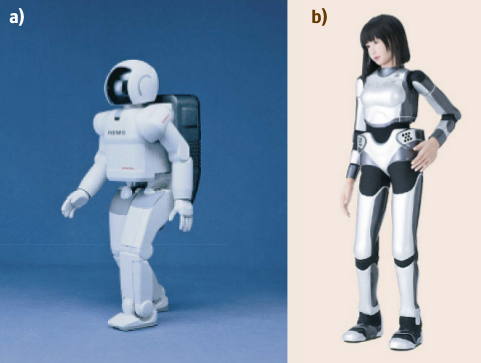
\includegraphics[scale=0.5]{images/asimov_and_HRP-4C.png}
	\caption{Diseño de robots humanoides (a) Asimov (2000); (b)HRP-4C (2009) (Tomado de: Siciliano and Khatib, 2016).}		
\end{figure}


		\textbf{Diseño conceptual}
El Humano cibernético o humanoide se define por las siguientes características:
\begin{itemize}
\item Tiene la apariencia y forma de un ser humano.
\item Puede caminar y moverse como un ser humano.
\item Puede interactuar con humanos usando reconocimiento de voz y de imágenes.
\end{itemize}
Tales robots pueden ser usados en la industria del entretenimiento, por ejemplo, en exhibiciones y presentaciones de moda. También se pueden usar como un simulador de humanos para evaluar dispositivos para humanos.\\

\subsection{Modelado y Control de Robots con Piernas}
	\textbf{Una Breve Historia de los Robots con piernas}\\
		Los robots con piernas controlados digitalmente empezaron a aparecer a finales de los 1960's. Entre los pioneros, Robert McGhee inicializó una serie de robots cuadrúpedos y hexápodos en \textit{University of South California}.\\

	\textbf{Dinámica del movimiento de los sistemas con piernas}\\
		Una de las mayores dificultades para hacer que un robot con extremidades camine o corra es mantener su balance: ¿Dónde debería caminar el robot?, ¿Cómo debería moverse su cuerpo a fin de moverse de manera segura en una dada dirección, incluso si hay fuertes perturbaciones?.\\ 

	\textbf{Análisis de estabilidad}\\
Para el control del sistema dinámico no lineal hay  un número de conceptos relativos para su seguridad y estabilidad los cuales son:

\begin{itemize}
\item \textit{Puntos fijos} : Representan las posturas estáticas en cuáles el robot puede estar de pie de manera segura.

\item \textit{Ciclos límites}: Proveen una natural extensión del análisis de los puntos fijos para movimientos de caminata periódica.

\item \textit{Viabilidad}: La viabilidad es un concepto de invarianza controlada, que analiza el conjunto de estados del cual el robot es capaz de mantenerse de pie. Desafortunadamente esta propiedad puede ser intratable para el cómputo.

\item \textit{Controlabilidad}: La controlabilidad provee una ligera noción de restricción de viabilidad, analizando el conjunto de estados del cual el robot es capaz de retornar a un particular punto fijo.

\item \textit{Estabilidad robusta}: Examina las propiedades del sistema considerando el "peor de los casos" de las perturbaciones. Por instancias, un controlador robusto debería ser capaz de garantizar que un punto fijo es estable incluso si la estimación de masa del tronco tiene un error del $\pm$10\%.

\item \textit{Estabilidad estocástica}: El análisis estocástico provee herramientas para investigar la probabilidad de caer. Para muchos modelos de perturbaciones en robots el sistema caerá eventualmente (con probabilidad uno), pero el análisis puede revelar la distribución del tiempo de vida metaestable.

\item \textit{Estabilidad de entrada-salida}: En este análisis se trata una particular perturbación como una entrada, un criterio de rendimiento como salida e intenta calcular una ganancia relativa o sensibilidad del rendimiento del robot debido a esta entrada.

\item \textit{Márgenes de estabilidad}: El análisis de robustez puede ser difícil. En la práctica, los diseñadores del control a menudo se conforman con que el sistema se mantenga cómodamente lejos de los límites de estabilidad determinista.		

\end{itemize}
%	\section{Aplicaciones en el juego de Futbol Soccer}
%	\section{Conceptos básicos de visión computacional}
%	\section{El filtro de Kalman}
%	\section{Trabajo relacionado}		
\chapter{ Segmentación de imágenes con base en color}
\section{Modelo de cámara Estenopeica \textit{(Pinhole)}}
De acuerdo con \cite{bradski2008learning} la visión es la detección de la luz del mundo. Esa luz empieza cuando un rayo emana desde una fuente hacia un objeto. Cuando la luz choca con el objeto, mucha de la luz es absorbida y la que no es absorbida, nosotros la podemos percibir como el color de la luz, de esta manera, la luz reflejada hace su camino hacia nuestra cámara. Esto es de particular importancia para la visión computacional.

El modelo más simple de cómo sucede el anterior fenómeno es el de la cámara estenopeica o \textit{pinhole}. Una cámara estenopeica se puede imaginar como una habitación sin ventanas en donde la luz únicamente entra por una pequeña apertura en el centro de la pared y que proyecta una imagen dentro de la habitación.

En cámara estenopeica se considera que sólo un rayo de luz entra desde un punto en particular, este punto es luego \textit{proyectado} sobre una superficie generalmente plana. Como resultado, la imagen en este plano (también llamado plano proyectivo), está siempre en el foco y su tamaño se relaciona a la distancia del objeto por un sólo parámetro de la cámara: \textit{la distancia focal}. La principal diferencia entre la imagen real y la que aparece en una cámara Pinhole, es que la imagen aparece invertida. 
	
El punto dentro del Pinhole es reinterpretado como el centro de proyección. Para este tipo de cámara, la distancia desde la abertura del Pinhole hacia la pantalla, es precisamente la distancia focal. Como puede verse en la Figura 2.1.\\
	
\begin{figure}
	\centering		
	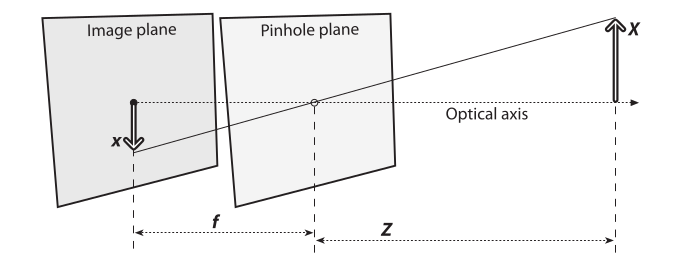
\includegraphics[scale=0.4]{images/pinhole.png}
	\caption{Esquema del modelo de cámara estenopeica (Tomado de: Bradski and Kaehler, 2008).}		
\end{figure}

En la Figura 2.1, $f$ es representada como la distancia focal de la cámara, $Z$ es la distancia de la cámara al objeto, $X$ es la longitud del objeto, y $x$ es la longitud de la la imagen proyectada en el plano. Dentro de la figura, se pueden ver dos triángulos semejantes los cuales cumplen que $-x/f = X/Z$, o expresado de otra manera:

\[x = -f \frac{X}{Z}\]
	
A fin de obtener ecuaciones equivalentes, pero sin signos negativos (correspondientes a la inversión de la imagen) se propone hacer un rearreglo en el cual se coloca al frente de un centro de proyección al plano proyectivo. Tal y como se ve en la Figura 2.2.
	
\begin{figure}
	\centering
	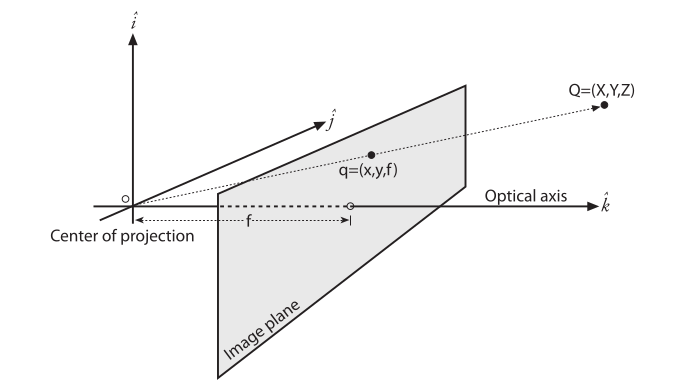
\includegraphics[scale=0.4]{images/rearreglo_pinhole.png}
    \caption{Rearreglo de una cámara estenopeica (Tomado de: Bradski and Kaehler, 2008).}
\end{figure} 

Con este nuevo cambio, el punto en el Pinhole es reinterpretado como el \textit{centro de proyección}, así cada rayo de luz deja un punto en el objeto distante y se dirije hacia el centro de proyección. El punto de intersección del plano proyectivo y el eje óptico es conocido como \textit{el punto principal}. El nuevo plano de imagen frontal es equivalente al anterior plano proyectivo, el cual la imagen del objeto distante tiene exactamente el mismo tamaño que en el esquema mostrado en la Figura 2.1, la diferencia es que en este caso la imagen no queda invertida, por lo tanto la relación de los triángulos quedaría de la siguiente manera: 
\[x/f = X/Z\]

Se podría pensar que que \textit{el punto principal} es equivalente al centro de la imagen, sin embargo, este centro usualmente no está en el eje óptico, es por eso que se introducen dos nuevos parámetros, $c_{x}$ y $c_{y}$ para modelar un posible desplazamiento (perpendicular al eje óptico) del centro de coordenadas en el plano de proyección. El resultado es que un punto Q en el mundo físico cuyas coordenadas son  (X,Y,Z) es proyectado dentro de la pantalla en una localización de pixeles dada por $(x_{screen},y_{screen})$ de acuerdo con las siguientes ecuaciones:

\[x_{screen}=f_{x}(\frac{X}{Z}) \quad + c_{x},\quad y_{screen}=f_{y}(\frac{Y}{Z}) + c_{y}\]	\\


Nótese que se han introducido dos diferentes distancias focales $f_{x}$ y $f_{y}$, la razón es porque generalmente los pixeles son rectangulares.
		
\section{Corrección de la distorsión}
Desafortunadamente una verdadera cámara pinhole no es una muy buena forma de obtener imágenes, ya que no reune suficiente luz en una rápida exposición para crear una imagen aproximada a la real. Es por eso que los ojos y las cámaras usan lentes para reunir más luz que la que estaría disponible en un solo punto.

\subsection{Geometría básica proyectiva}
La relación que mapea los puntos $Q_{i}$ en el mundo físico con coordenadas $(X_{i},Y_{i},Z_{i})$ a los puntos en el plano de proyección con coordenadas $(x_{i},y_{i})$ es llamada una \textit{transformación proyectiva}. Cuando se trabaja con estas transformaciones es conveniente usar las \textit{coordenada homogéneas}. El plano de imagen es el espacio proyectado y tiene dos dimensiones, con lo que se pueden representar puntos en el plano como un vector tridimensional $q=(q_{1},q_{2},q_{3})$ ó $q=(x, y, w)$, en donde w es la orientación. Una forma de hacer un arreglo con los parámetros que definen a la cámara $f_{x},f_{y},c_{x}$ y $c_{y}$ dentro de una matriz de 3x3 es la llamada \textit{matriz de parámetros intrínsecos}. La proyección $q$ de los puntos del mundo físico en el plano de la imagen se puede calcular como: 
\[q=MQ\]
donde
\[q=
\begin{bmatrix}
x\\ 
y\\
w 
\end{bmatrix}\;,\;M=
\begin{bmatrix}
f_{x} & 0 & c_{x}\\ 
0     &f_{y}&c_{y} \\
0     & 0 & 1
\end{bmatrix}\;,\;Q=
\begin{bmatrix}
X\\
Y\\
Z
\end{bmatrix}
\]
\subsection{Distorsión de las lentes}
La estimación de los parámetros internos es importante en la calibración de las cámaras \cite{bradski2008learning}.


Dada la manufactura y diversos factores, las lentes no son perfectas, es por eso que se introducen dos nuevos conceptos a la distorsión de las lentes, las \textit{Distorsiones radiales} y las \textit{Distorsiones tangenciales}. Las primeras surgen como resultado de la forma de las lentes y las segundas como resultado del proceso de ensamblado de la cámara.

La distorsión radial es notable cuando la imagen se hace más pequeña conforme está más cerca de los pixeles de los extremos, esto es más evidente en las cámaras de baja calidad, sin embargo es un hecho que todas la tienen. En la práctica, se puede caracterizar esta distorsión con la serie de Taylor, las ecuaciones son:
\[x_{corregida} = x(1+k_1r^2+k_2r^4+k_3r^6)\]
\[y_{corregida} = y(1+k_1r^2+k_2r^4+k_3r^6)\]

En donde $(x,y)$ son las coordenadas de la imagen, \textit{r} es la distancia del punto de la imagen al centro y las constantes $k_1$, $k_2$ y $k_3$ son parámetros que están relacionados a cada cámara en específico.

Las \textit{Distorsiones tangenciales} son ocacionadas por no tener paralelas las lentes con el plano de la imagen. Para obtener expresiones que ayuden a corregir este tipo de distorsión se introducen dos parámetros: $p_{1}$ y $p_{2}$ dentro de las siguientes ecuaciones:
\[x_{corrected} = x + [2p_1y+p_2(r^2+2x^2)]\]
\[y_{corrected} = y + [p_1(r^2+2y^2)+2p_2x]\]

Para poder hacer una corrección automática de todas las distorsiones, las herramientas de OpenCV usan los cinco parámetros antes mencionados dentro de una matriz de 1x5 llamada \textit{matriz de coeficientes de distorsión}, en donde cada parámetro se acomoda de la siguiente forma:
\[[k_1 \quad k_2 \quad p_1 \quad p_2 \quad k_3]\]
\section{Los espacios de color RGB y HSV}
Citando a \cite{gonzalez2002digital} se usa el color para el procesamiento de imagenes debido a que el color es un muy buen descriptor para la identificación de objetos (mejor que otro tipo de segmentación como el de escala de grises).
\\

\textbf{Percepción del color}\\
Según \cite{agoston2005computer} en el caso más simple, la percepción del color tiene tres características principales llamadas \textit{matiz, saturación y brillo}. 
\begin{itemize}
\item \textit{Matiz (Hue):} La matiz es un descriptor de qué tan combinados están los colores unitarios entre sí (si se entiende por color unitario a los colores rojo, amarillo, verde y azul).

\item \textit{Saturación (Saturation): } La saturación es la percepción de la relativa carga de color que tiene la matiz. Se puede decir que la saturación es una medida de qué tan puro es un color si éste es diluido en blanco.

\item \textit{Brillo: (Brightness)} El brillo es un atributo de la iluminación en la cual un objeto no aislado se ve afectado, es notable cuando un objeto de un  mismo color cambia su tonalidad debido a las variaciones de iluminación de su entorno.
\end{itemize}

\textbf{Espacios de color}
El \textit{espacio de color} es un modelo utilizado para facilitar la especificación de cualquier color de una manera estandarizada. Uno de los sistemas más conocidos, es el espacio de color RGB (por sus siglas en inglés red, green y blue), que está basado en un sistema coordenado ortogonal (como se observa en la Figura 2.3) en donde la escala de los colores primarios está cada uno en los ejes.

El espacio de color \textit{HSV (Hue-Saturation-Value)} es especificado por por tres números que corresponden a la matiz (Hue), saturación (saturation) y el valor (value). La matiz corresponde a un ángulo de 0 a 360 grados. La saturación se toma entre valores de 0 a 1 que miden la salida de la matiz del blanco. El valor (value) que va del 0 al 1 mide la salida de la matiz del negro o \textit{color de energía cero}, véase la Figura 2.4 en donde se observa el modelo tridimencional de este espacio.

\begin{figure}
	\centering		
	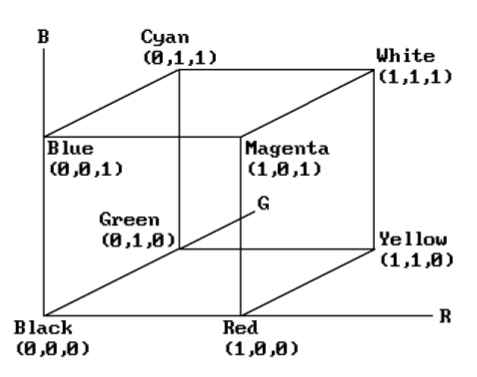
\includegraphics[scale=0.4]{images/RGB_model.png}
	\caption{Modelo tridimensional del espacio de color RGB (Foto tomada de: \cite{agoston2005computer}).}		
\end{figure}

\begin{figure}
	\centering		
	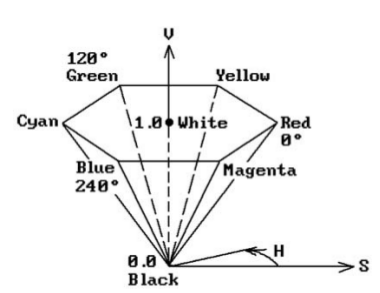
\includegraphics[scale=0.6]{images/hexacono_HSV.png}
	\caption{Modelo tridimensional del espacio de color HSV (Foto tomada de: \cite{agoston2005computer}).}		
\end{figure}

Tanto el espacio de color RGB y el HSV pueden representar la totalidad de los colores del espectro de luz visible, no obstante para el procesamiento de imágenes se utiliza el HSV ya que es una forma más sencilla para segmentar colores y es una forma más parecida a la que los seres humanos percibimos los colores.

\section{Operadores morfológicos}	
La gran mayoría de las veces, cuando se hace procesamiento de imágenes, se necesitan procesos para eliminar el ruido circundante y dejar al elemento de interés aislado, para esto OpenCV tiene provee los \textit{operadores morfológicos}. Los operadores básicos son \textit{erosión y dilatación} y tienen una gran variedad de características para realizar su función.

La \textit{dilatación} es una convolución sobre una región de la imagen a la que comunmente se le llama \textit{kernel}, la cual puede tener cualquier forma o tamaño y tiene definido un \textit{punto de anclaje}. La mayor parte de las veces como un cuadrado o un disco cuyo \textit{punto de anclaje} está en el centro. El \textit{kernel} puede ser pensado como como una plantilla o una máscara y su efecto para la dilatación es el de ensanchar un \textit{máximo local}, cada ensanchamiento hace que la figura total se ensanche de una manera uniforme, tal y como se ve en la Figura 2.5.
\begin{figure}
	\centering		
	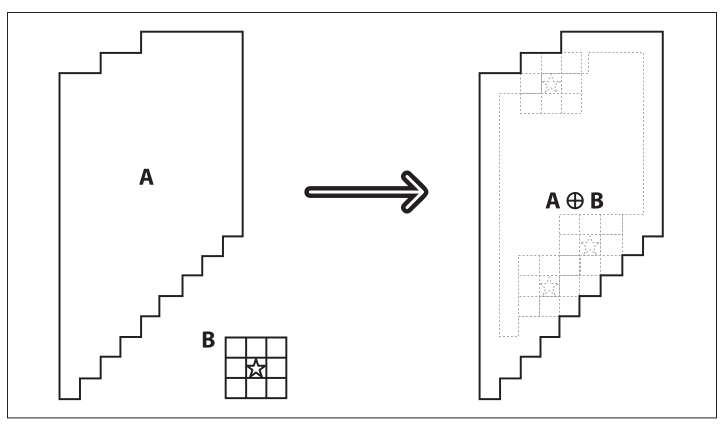
\includegraphics[scale=0.4]{images/dilatacion.png}
	\caption{Efecto de la operación morfológica de la dilatación}		
\end{figure}
 La \textit{erosión} es la operación inversa a la dilatación, ya que opera sobre el mínimo local 

\chapter{Estimación de posición y velocidad}
	\section{Cálculo de la posición del objeto de interés}
Tal como se observa en la simulación de Gazebo (Figura 3.1), se decidió usar un sistema ortogonal derecho en la base de los pies como sistema de referencia que gobernará a todo el modelo.

\begin{figure}
	\centering		
	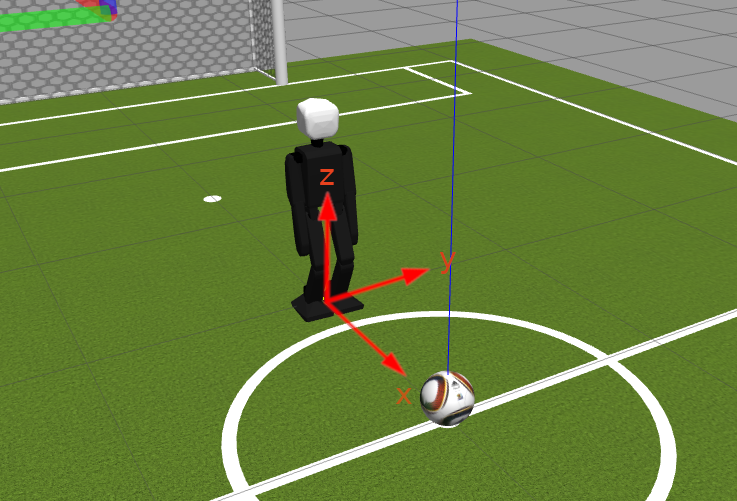
\includegraphics[scale=2]{images/robot_ejes.png}
	\caption{Representación del sistema de referencia usado en el robot.}		
\end{figure}

La cámara está localizada en la cabeza del humanoide, por lo que su centro
de visión se puede representar por un eje que va de la cámara al centroide del 
objeto, en este caso un balón de football.
Para estimar la posición de un objeto que cruce por el centro de visión de la
cámara se necesita establecer un vector unitario, a este vector se le conoce
como \textit{look at}, tal como se observa en la imagen (Figura 3.2)

\begin{figure}
	\centering		
	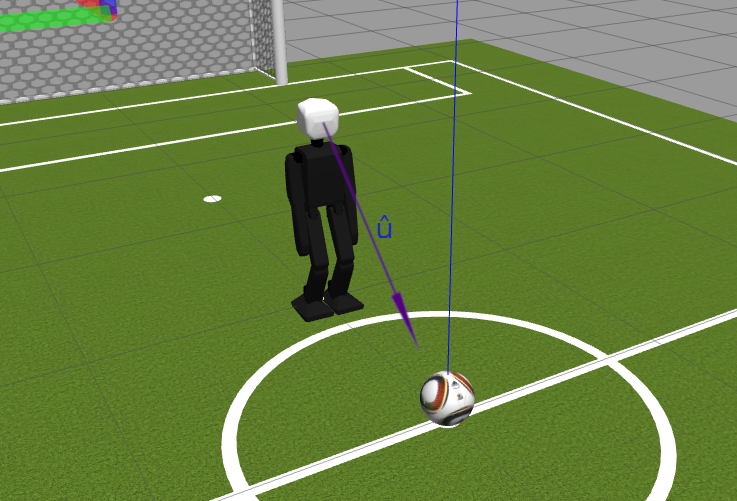
\includegraphics[scale=2]{images/robot_lookat.png}
	\caption{Representación del vector \textit{look at} utilizado en visión computacional.}		
\end{figure}


Una vez teniendo el sistema de referencia y la posición inicial de nuestro vector de interés, se procede a hacer un desarrollo matemático. Empezando por nombrar al vector \textit{look at} con la siguiente expresión:

\[\hat{u} = (u_x, u_y, u_z)\]
 
Para obtener la ecuación vectorial de la recta paralela al vector \textit{look at} se toma un punto que contenga la recta, en este caso la posición de la cabeza en donde se encuentra la cámara:
\[r(\lambda) = (r_x, r_y, r_z)\quad +\quad \lambda (u_x, u_y, u_z)...............................................................(1)\]

En donde $(r_x, r_y, r_z)$ es la posición en el espacio de la cámara utilizada, referida al sistema de referencia anteriormente mencionado. Se considera que el objetivo siempre estará en el suelo, por lo que el punto de intersección de la ecuación de la recta con el suelo hacen que la variable de altura sea igual a cero, conforme a la siguiente expresión:
\[r = (x, y, 0) = (r_x, r_y, r_z) + \lambda (u_x, u_y, u_z)\]
Despejando lamda del tercer término de la expresión anterior se puede obtener fácilmente lamda:
\[\lambda = -\frac{r_z}{u_z}\]

De esta manera, substituyendo lamnda en la ecuación (1), se obtiene:
\[x = r_x-\frac{r_z u_x}{u_z}\]
\[y = r_y-\frac{r_z u_y}{u_z}\]

Ya teniendo estas expresiones se procede a sustituir al vector unitario \textit{look at} con coordenadas esféricas, tal y como se observa en la siguiente expresión:
\[\hat{u}=(u_x, u_y, u_z)=(\sin{ \theta}\cos{\varphi},\sin{\theta}\sin{ \varphi},\cos{\theta})..............................................(2)\]

Sustituyendo la expresión (2) dentro de los valores $x$ y $y$ quedan como:
\[x=r_x - \frac{r_z \sin{ \theta} \cos{\varphi}}{\cos{\theta}}\]
\[y=r_y - \frac{r_z \sin{\theta} \sin{ \varphi}}{\cos{\theta}}\]

Utilizando la identidad trigonométrica:
\[\tan{\theta} = \frac{\sin{\theta}}{\cos{\theta}}\]

Por lo tanto, las ecuaciones para obtener la posición del objetivo siempre y cuando $z=0$ quedan:
\[x=r_x - r_z \tan{\theta}  \cos{\varphi}\]
\[y=r_y - r_z \tan{\theta} \sin{\varphi}\]
%	\chapter{Implementación}
%	\chapter{Resultados}
%\bibliographystyle{apacite}
\bibliographystyle{ieeetr}
\bibliography{References}
\end{document}
